\section{Embedded control system}

It is imperative to create a controller which minimizes the effects of communication delay. Therefore the aim was to implement as much of the motion control on the embedded system as possible. The human operator  inputs the required position by moving the GT. These positions are sent as position reference to the sbRIO. 
The sbRIO has an implemented cascade position-speed-current control, see \figref{cascade_fig}, which takes care of the EndoWrist positioning tasks. The P position control that tracks the setpoint is running on the sbRIO FPGA. The FPGA sends the speed reference to the Escon controller in the form of PWM signals. The Escon controller is running the PI speed control with inner PI current control loop. The inner loops are faster than the outer loops.

The chosen controller parameters:

\begin{center}
	\begin{tabular}{ c | c | c | c }
		\hline
		Controller type & P gain & I time constant & Sampling rate \\ \hline
		Position controller & 10 & 0 & 2 kHz \\ \hline
		Speed controller & 426 & 28 ms & 5.36 kHz \\ \hline
		Position controller & 1121 & $38 \mu s$ & 53.6 kHz \\ \hline
	\end{tabular}
\end{center}

The speed and current controller parameters were calibrated automatically by ESCON Studio. The program queries the motor parameters, desired current limits and maximum acceleration values and calculates the controller parameters based on those. The EndoWrist can not handle high speeds and high acceleration, thus speed was not the main priority in tuning the position PID control. We focused on precision and avoiding overshoot. By running experiments, we decided upon a P controller of 10 for each motor. A lower gain would result in slower motion, a higher gain would result in overshoots. The EndoWrist-motor system has inherent damping in the form of friction, inertia and elasticity, thus the system is stable even without integral and differential controller. The following graph shows experiments with free-running EndoWrist. The setpoints square signals moving jumping between the limits the EndoWrist can move between. This is a movement that would never happen in normal operation.

% This file was created by matlab2tikz.
%
%The latest updates can be retrieved from
%  http://www.mathworks.com/matlabcentral/fileexchange/22022-matlab2tikz-matlab2tikz
%where you can also make suggestions and rate matlab2tikz.
%
\definecolor{mycolor1}{rgb}{0.00000,0.44700,0.74100}%
\definecolor{mycolor2}{rgb}{0.85000,0.32500,0.09800}%
%
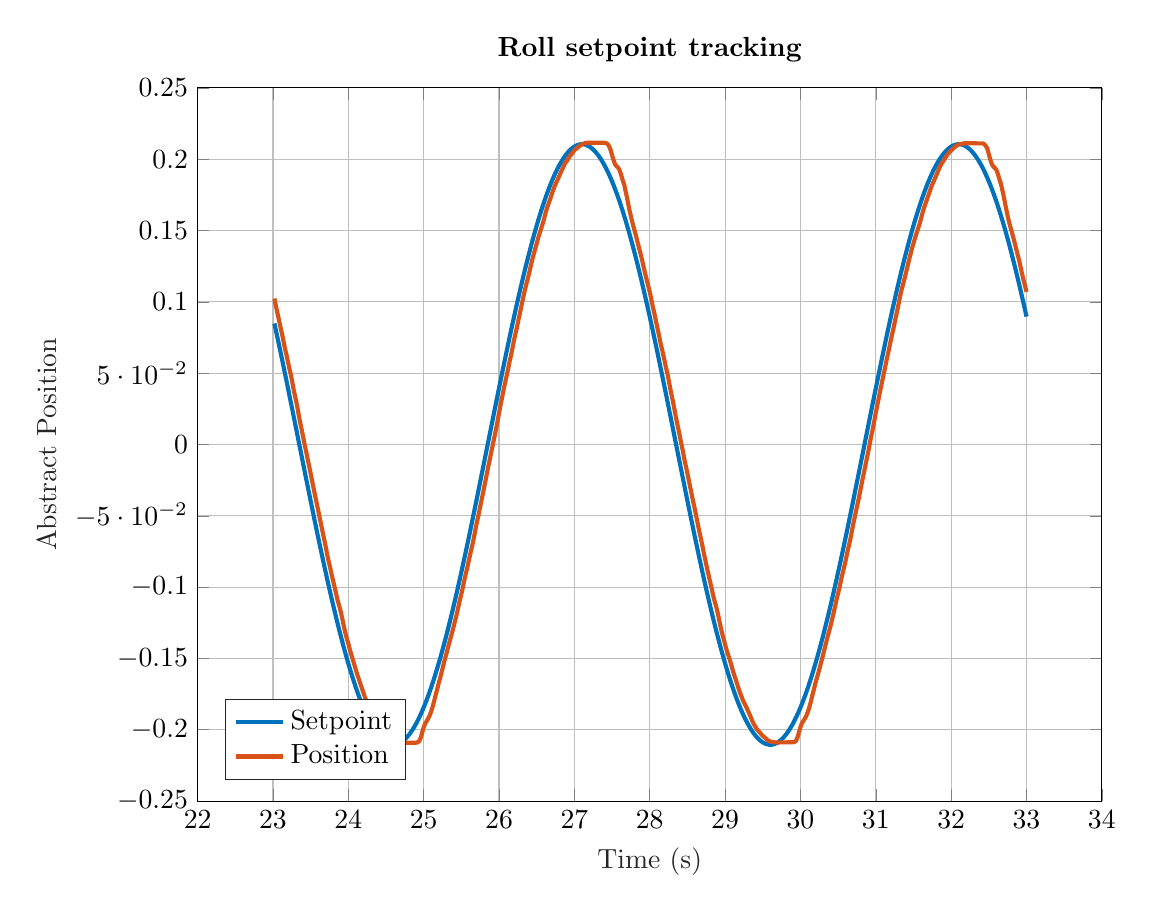
\begin{tikzpicture}

\begin{axis}[%
width=4.521in,
height=3.566in,
at={(0.758in,0.481in)},
scale only axis,
xmin=22,
xmax=34,
xlabel style={font=\color{white!15!black}},
xlabel={Time (s)},
ymin=-0.25,
ymax=0.25,
ylabel style={font=\color{white!15!black}},
ylabel={Abstract Position},
axis background/.style={fill=white},
title style={font=\bfseries},
title={Roll setpoint tracking},
xmajorgrids,
ymajorgrids,
legend style={at={(0.03,0.03)}, anchor=south west, legend cell align=left, align=left, draw=white!15!black}
]
\addplot [color=mycolor1, line width=1.5pt]
  table[row sep=crcr]{%
23.0191555	0.084822410000001\\
23.0791626	0.0700672700000027\\
23.11917114	0.0600040500000034\\
23.19929695	0.0394487000000012\\
23.3391819	0.0026454799999982\\
23.47919846	-0.034239399999997\\
23.57920647	-0.0600040500000034\\
23.65921402	-0.0799534900000012\\
23.71923447	-0.0943964599999987\\
23.77923203	-0.108303059999997\\
23.83923912	-0.121594250000001\\
23.87924385	-0.13007571\\
23.93925476	-0.14217532\\
23.9792614	-0.149796989999999\\
24.01925659	-0.157040240000001\\
24.05926514	-0.1638868\\
24.09938622	-0.170319360000001\\
24.1392746	-0.176321700000003\\
24.17927551	-0.181878609999998\\
24.21928978	-0.186976090000002\\
24.25928879	-0.191601249999998\\
24.2994175	-0.195742410000001\\
24.33930206	-0.199389109999998\\
24.37930679	-0.202532140000002\\
24.41931152	-0.205163550000002\\
24.45931435	-0.207276700000001\\
24.49943924	-0.20886625\\
24.53932953	-0.209928179999999\\
24.57933235	-0.210459829999998\\
24.61933899	-0.210459829999998\\
24.65933609	-0.209928179999999\\
24.69947052	-0.20886625\\
24.73935127	-0.207276700000001\\
24.77935219	-0.205163550000002\\
24.81936455	-0.202532140000002\\
24.85939026	-0.199389109999998\\
24.89950562	-0.195742410000001\\
24.93938637	-0.191601249999998\\
24.97940445	-0.186976090000002\\
25.01939392	-0.181878609999998\\
25.05941391	-0.176321700000003\\
25.09952736	-0.170319360000001\\
25.13941765	-0.1638868\\
25.17942429	-0.157040240000001\\
25.21941948	-0.149796989999999\\
25.2595253	-0.14217532\\
25.29954147	-0.134194520000001\\
25.33945274	-0.12587473\\
25.37944412	-0.117236980000001\\
25.41944885	-0.108303059999997\\
25.45945358	-0.0990955600000021\\
25.51947403	-0.084822410000001\\
25.57947159	-0.0700672700000027\\
25.61948204	-0.0600040500000034\\
25.69965935	-0.0394487000000012\\
25.89969635	0.0132190599999973\\
25.95955086	0.0290084800000017\\
26.03957939	0.0497892599999972\\
26.09970474	0.0650562100000016\\
26.13957214	0.0750340800000018\\
26.17958832	0.084822410000001\\
26.23957825	0.0990955600000021\\
26.27958679	0.108303059999997\\
26.33958435	0.121594250000001\\
26.37959862	0.13007571\\
26.43959999	0.14217532\\
26.47961998	0.149796989999999\\
26.51965904	0.157040240000001\\
26.559618	0.1638868\\
26.59978867	0.170319360000001\\
26.63961983	0.176321700000003\\
26.67969131	0.181878609999998\\
26.71968079	0.186976090000002\\
26.7596817	0.191601249999998\\
26.79981041	0.195742410000001\\
26.83969688	0.199389109999998\\
26.8796978	0.202532140000002\\
26.91968918	0.205163550000002\\
26.95970345	0.207276700000001\\
26.9998188	0.20886625\\
27.03972244	0.209928179999999\\
27.07970428	0.210459829999998\\
27.11972046	0.210459829999998\\
27.15972137	0.209928179999999\\
27.19987488	0.20886625\\
27.23973846	0.207276700000001\\
27.27972794	0.205163550000002\\
27.31974983	0.202532140000002\\
27.3597641	0.199389109999998\\
27.39987946	0.195742410000001\\
27.43976212	0.191601249999998\\
27.47976685	0.186976090000002\\
27.51978683	0.181878609999998\\
27.55976677	0.176321700000003\\
27.59990501	0.170319360000001\\
27.63977814	0.1638868\\
27.67980003	0.157040240000001\\
27.71977997	0.149796989999999\\
27.75979042	0.14217532\\
27.79992867	0.134194520000001\\
27.83981323	0.12587473\\
27.87981415	0.117236980000001\\
27.91983032	0.108303059999997\\
27.97982025	0.0943964599999987\\
28.01981544	0.084822410000001\\
28.07985115	0.0700672700000027\\
28.11987686	0.0600040500000034\\
28.19997215	0.0394487000000012\\
28.31985855	0.00793477999999936\\
28.47991753	-0.034239399999997\\
28.57987976	-0.0600040500000034\\
28.65989304	-0.0799534900000012\\
28.71993256	-0.0943964599999987\\
28.75995255	-0.10373207\\
28.80004501	-0.112805639999998\\
28.8399334	-0.121594250000001\\
28.87992287	-0.13007571\\
28.93993759	-0.14217532\\
28.97994614	-0.149796989999999\\
29.01994705	-0.157040240000001\\
29.05997849	-0.1638868\\
29.10009575	-0.170319360000001\\
29.13996696	-0.176321700000003\\
29.17998505	-0.181878609999998\\
29.21994209	-0.186976090000002\\
29.25997353	-0.191601249999998\\
29.30012321	-0.195742410000001\\
29.34000587	-0.199389109999998\\
29.3800087	-0.202532140000002\\
29.41999435	-0.205163550000002\\
29.46001816	-0.207276700000001\\
29.50014114	-0.20886625\\
29.54003143	-0.209928179999999\\
29.58001518	-0.210459829999998\\
29.62005615	-0.210459829999998\\
29.66002274	-0.209928179999999\\
29.70015717	-0.20886625\\
29.74006462	-0.207276700000001\\
29.78003311	-0.205163550000002\\
29.82004356	-0.202532140000002\\
29.86007118	-0.199389109999998\\
29.90019608	-0.195742410000001\\
29.94006538	-0.191601249999998\\
29.98004532	-0.186976090000002\\
30.02007484	-0.181878609999998\\
30.06008911	-0.176321700000003\\
30.10021591	-0.170319360000001\\
30.14009857	-0.1638868\\
30.18009949	-0.157040240000001\\
30.22017097	-0.149796989999999\\
30.26011658	-0.14217532\\
30.30026627	-0.134194520000001\\
30.36011124	-0.121594250000001\\
30.40029907	-0.112805639999998\\
30.4601326	-0.0990955600000021\\
30.52017593	-0.084822410000001\\
30.58013344	-0.0700672700000027\\
30.62013245	-0.0600040500000034\\
30.70029259	-0.0394487000000012\\
30.84021378	-0.0026454799999982\\
30.980196	0.034239399999997\\
31.08020401	0.0600040500000034\\
31.1602459	0.0799534900000012\\
31.22019577	0.0943964599999987\\
31.28022957	0.108303059999997\\
31.34022331	0.121594250000001\\
31.38021278	0.13007571\\
31.44024277	0.14217532\\
31.48025322	0.149796989999999\\
31.520298	0.157040240000001\\
31.56042099	0.1638868\\
31.60041428	0.170319360000001\\
31.64028549	0.176321700000003\\
31.68028259	0.181878609999998\\
31.72029877	0.186976090000002\\
31.76030731	0.191601249999998\\
31.80044556	0.195742410000001\\
31.84035492	0.199389109999998\\
31.88029289	0.202532140000002\\
31.92034912	0.205163550000002\\
31.96029282	0.207276700000001\\
32.00043488	0.20886625\\
32.04032898	0.209928179999999\\
32.08035278	0.210459829999998\\
32.12031555	0.210459829999998\\
32.16034317	0.209928179999999\\
32.20049286	0.20886625\\
32.24038315	0.207276700000001\\
32.28037262	0.205163550000002\\
32.32038116	0.202532140000002\\
32.36040878	0.199389109999998\\
32.40048218	0.195742410000001\\
32.44039536	0.191601249999998\\
32.48039627	0.186976090000002\\
32.5204277	0.181878609999998\\
32.56040192	0.176321700000003\\
32.60052109	0.170319360000001\\
32.64037704	0.1638868\\
32.68041992	0.157040240000001\\
32.72045135	0.149796989999999\\
32.7604332	0.14217532\\
32.8005867	0.134194520000001\\
32.86040115	0.121594250000001\\
32.90053558	0.112805639999998\\
32.96042633	0.0990955600000021\\
33.00058746	0.0896377400000006\\
};
\addlegendentry{Setpoint}

\addplot [color=mycolor2, line width=1.5pt]
  table[row sep=crcr]{%
23.0191555	0.102349680000003\\
23.03915405	0.0969758999999968\\
23.0992794	0.0824253899999974\\
23.11917114	0.0777130000000028\\
23.15916443	0.0672961499999971\\
23.17917252	0.0627491199999994\\
23.21917725	0.0529109800000001\\
23.23917961	0.04844662\\
23.27918243	0.037120360000003\\
23.29930305	0.0324906499999997\\
23.31919098	0.0275302399999973\\
23.3391819	0.0214124100000035\\
23.35918236	0.0157906199999971\\
23.37919235	0.0109128900000002\\
23.41919327	0.000165350000003173\\
23.43920135	-0.00462971000000323\\
23.459198	-0.0100034800000017\\
23.47919846	-0.0149638899999971\\
23.55920982	-0.0359629299999966\\
23.59934044	-0.0458837400000007\\
23.6192131	-0.0511748400000016\\
23.67922783	-0.0663867399999987\\
23.69934082	-0.0714298299999996\\
23.71923447	-0.0771342899999965\\
23.73923111	-0.0820120200000005\\
23.75923157	-0.086393710000003\\
23.77923203	-0.0913541099999975\\
23.83923912	-0.104829889999998\\
23.8592453	-0.109624940000003\\
23.87924385	-0.113097209999999\\
23.89936638	-0.117230890000002\\
23.91924667	-0.121943270000003\\
23.93925476	-0.127069030000001\\
23.95925522	-0.131864090000001\\
23.9792614	-0.135915089999997\\
23.99937439	-0.139470039999999\\
24.01925659	-0.143686379999998\\
24.05926514	-0.150796290000002\\
24.11927795	-0.161378489999997\\
24.21928978	-0.177003759999998\\
24.23929024	-0.17973198\\
24.27929878	-0.183948319999999\\
24.37930679	-0.195853290000002\\
24.39942551	-0.197754789999998\\
24.41931152	-0.199408249999998\\
24.47932053	-0.2027152\\
24.51931763	-0.205030049999998\\
24.57933235	-0.20800629\\
24.59946823	-0.20858501\\
24.63933563	-0.209081050000002\\
24.69947052	-0.209163709999999\\
24.89950562	-0.209081050000002\\
24.9193821	-0.20883302\\
24.93938637	-0.20800629\\
24.9593811	-0.205856789999999\\
24.99950981	-0.198333499999997\\
25.01939392	-0.195770619999998\\
25.05941391	-0.192132989999998\\
25.07941818	-0.189983490000003\\
25.09952736	-0.187172590000003\\
25.11941338	-0.183700309999999\\
25.13941765	-0.179814669999999\\
25.15943146	-0.17551564\\
25.17942429	-0.17163\\
25.19954681	-0.167248290000003\\
25.21941948	-0.16352801\\
25.23942566	-0.159477010000003\\
25.27942657	-0.150878970000001\\
25.29954147	-0.147158670000003\\
25.31944466	-0.142942310000002\\
25.37944412	-0.131368039999998\\
25.39957237	-0.127317060000003\\
25.41944885	-0.122935349999999\\
25.43946648	-0.118801679999997\\
25.45945358	-0.114171970000001\\
25.47947884	-0.109211569999999\\
25.49957657	-0.104912550000002\\
25.51947403	-0.100282849999999\\
25.53948212	-0.0951570900000007\\
25.55951691	-0.0904447099999999\\
25.57947159	-0.0863110399999982\\
25.59960938	-0.0811852799999997\\
25.61948204	-0.0764728999999988\\
25.63947678	-0.0720085399999988\\
25.65950775	-0.0672134799999995\\
25.69965935	-0.0561352400000033\\
25.71951675	-0.05150553\\
25.77954102	-0.0360456000000013\\
25.79967308	-0.0309198499999965\\
25.85951996	-0.0149638899999971\\
25.95955086	0.0104995200000033\\
25.97954559	0.0161213100000026\\
25.99969482	0.0219911300000035\\
26.01956367	0.0274475699999996\\
26.03957939	0.0326560000000029\\
26.05957413	0.038112439999999\\
26.11956024	0.0527456299999969\\
26.13957214	0.0579540600000001\\
26.15955734	0.0625837700000034\\
26.17958832	0.0677921999999995\\
26.19974518	0.0734139899999988\\
26.23957825	0.0825080600000021\\
26.25958061	0.0878818300000006\\
26.27958679	0.0925942100000015\\
26.31958199	0.102680370000002\\
26.33958435	0.107475430000001\\
26.35961342	0.111857120000003\\
26.37959862	0.115742769999997\\
26.39978218	0.120041790000002\\
26.41959763	0.124836850000001\\
26.43959999	0.129218530000003\\
26.47961998	0.137155180000001\\
26.49975395	0.140710149999997\\
26.51965904	0.144843799999997\\
26.57962227	0.154764610000001\\
26.59978867	0.158650280000003\\
26.61962128	0.162783939999997\\
26.63961983	0.166173550000003\\
26.67969131	0.17212602\\
26.69979858	0.175432970000003\\
26.71968079	0.178491880000003\\
26.73966599	0.181220099999997\\
26.81968689	0.190644880000001\\
26.85968971	0.195274589999997\\
26.8796978	0.197424099999999\\
26.89981651	0.198746870000001\\
26.93969345	0.202053820000003\\
26.97970009	0.204782039999998\\
26.9998188	0.206270160000003\\
27.07970428	0.209742429999999\\
27.11972046	0.210899859999998\\
27.15972137	0.211561250000003\\
27.39987946	0.211478589999999\\
27.41974258	0.211313220000001\\
27.43976212	0.210651839999997\\
27.45976257	0.209163709999999\\
27.47976685	0.20660084\\
27.51978683	0.199242900000002\\
27.53976059	0.196432010000002\\
27.55976677	0.195109250000002\\
27.57977867	0.194117159999998\\
27.59990501	0.192298350000002\\
27.6197834	0.189156760000003\\
27.63977814	0.185436439999997\\
27.65979767	0.182460200000001\\
27.67980003	0.177499820000001\\
27.69993019	0.172787409999998\\
27.71977997	0.16716564\\
27.73979187	0.162287910000003\\
27.75979042	0.157740859999997\\
27.77978325	0.153607190000002\\
27.81982803	0.145918559999998\\
27.83981323	0.141536879999997\\
27.87981415	0.133434880000003\\
27.89992714	0.128970500000001\\
27.93980408	0.119628409999997\\
27.99995804	0.106979389999999\\
28.01981544	0.102101660000002\\
28.03981781	0.09689324\\
28.05982971	0.092263520000003\\
28.09995842	0.0821773699999966\\
28.11987686	0.0772996299999988\\
28.13983154	0.0720085399999988\\
28.17984009	0.0628317899999971\\
28.21988106	0.0529936599999985\\
28.23985672	0.0483639400000015\\
28.27983856	0.037120360000003\\
28.3000145	0.0323252999999966\\
28.31985855	0.0269515299999981\\
28.33985138	0.0213297399999988\\
28.35985947	0.0159559700000003\\
28.37986183	0.0109128900000002\\
28.41988564	0.000330689999998413\\
28.43987274	-0.00471238000000085\\
28.45988464	-0.0104168499999986\\
28.49998093	-0.0201723099999995\\
28.5398941	-0.0306718300000028\\
28.55990982	-0.035880259999999\\
28.60004807	-0.0458010700000031\\
28.61990929	-0.0509268200000008\\
28.63990402	-0.0563005899999993\\
28.65989304	-0.061426339999997\\
28.67989922	-0.0661387199999979\\
28.70003891	-0.0712644800000035\\
28.71993256	-0.0766382400000012\\
28.75995255	-0.086559059999999\\
28.80004501	-0.0959838300000015\\
28.81992149	-0.100448190000002\\
28.8399334	-0.105325919999999\\
28.85992241	-0.109707610000001\\
28.87992287	-0.113179899999999\\
28.90008354	-0.117644259999999\\
28.91993523	-0.122521990000003\\
28.93993759	-0.12764774\\
28.95993042	-0.132277440000003\\
29.01994705	-0.144017069999997\\
29.05997849	-0.15063095\\
29.0799942	-0.154103229999997\\
29.10009575	-0.157988879999998\\
29.11994553	-0.161461160000002\\
29.13996696	-0.164520070000002\\
29.17998505	-0.171216620000003\\
29.20013809	-0.174275530000003\\
29.23999405	-0.17973198\\
29.27997208	-0.183865670000003\\
29.34000587	-0.191058249999998\\
29.36000061	-0.193703790000001\\
29.3800087	-0.195935980000002\\
29.41999435	-0.199490930000003\\
29.48002243	-0.203128560000003\\
29.50014114	-0.204368670000001\\
29.5200119	-0.205112730000003\\
29.56004143	-0.207096890000003\\
29.60014915	-0.208254310000001\\
29.64002037	-0.208750350000003\\
29.68003845	-0.208915699999999\\
29.90019608	-0.208750350000003\\
29.92011642	-0.20858501\\
29.94006538	-0.20775828\\
29.9600811	-0.205608759999997\\
30.00018692	-0.198168160000002\\
30.02007484	-0.195357260000002\\
30.06008911	-0.19205032\\
30.08009148	-0.189983490000003\\
30.10021591	-0.187255260000001\\
30.12007904	-0.183865670000003\\
30.14009857	-0.17997999\\
30.16010284	-0.175432970000003\\
30.18009949	-0.171464640000004\\
30.20022011	-0.167082950000001\\
30.24011803	-0.159725029999997\\
30.30026627	-0.147654709999998\\
30.32013321	-0.143190339999997\\
30.36011124	-0.134923010000001\\
30.40029907	-0.127069030000001\\
30.4601326	-0.113510589999997\\
30.48015213	-0.108550180000002\\
30.50025749	-0.10441651\\
30.52017593	-0.0997867999999968\\
30.54016113	-0.0947437199999968\\
30.56018829	-0.0902793599999967\\
30.58013344	-0.0860630099999966\\
30.60030365	-0.0812679599999981\\
30.62013245	-0.0760595400000028\\
30.66015244	-0.0670481300000034\\
30.70029259	-0.0559699000000009\\
30.780159	-0.036293630000003\\
30.82019997	-0.025546079999998\\
30.90029144	-0.00496040000000164\\
30.94021988	0.00611783000000088\\
30.96017838	0.0108302200000026\\
30.980196	0.0164520100000018\\
31.00031853	0.0223218200000019\\
31.06018448	0.038112439999999\\
31.12021065	0.0531590000000008\\
31.14019394	0.058367429999997\\
31.18021011	0.0679575400000019\\
31.20035934	0.0733313100000004\\
31.24022675	0.0826734099999982\\
31.26019287	0.0878818300000006\\
31.28022957	0.0927595599999975\\
31.30033493	0.0978853100000023\\
31.32023621	0.103176410000003\\
31.34022331	0.107971470000003\\
31.3602562	0.111857120000003\\
31.38021278	0.116073460000003\\
31.40035629	0.12012447\\
31.44024277	0.129135859999998\\
31.48025322	0.137403210000002\\
31.50040054	0.140958159999997\\
31.520298	0.144678470000002\\
31.5802803	0.15451659\\
31.60041428	0.158236909999999\\
31.62028503	0.162370559999999\\
31.64028549	0.165925530000003\\
31.74024773	0.181054760000002\\
31.80044556	0.188330020000002\\
31.82031822	0.190727549999998\\
31.84035492	0.193373100000002\\
31.8602562	0.195605280000002\\
31.88029289	0.197506769999997\\
31.90040207	0.198912219999997\\
31.92034912	0.200813709999998\\
31.94027901	0.202467169999998\\
31.98027229	0.205112730000003\\
32.06033325	0.209081050000002\\
32.10045242	0.210321139999998\\
32.18030548	0.211230559999997\\
32.42037964	0.211065220000002\\
32.44039536	0.210486500000002\\
32.46037674	0.209329070000003\\
32.48039627	0.207427580000001\\
32.5204277	0.199573610000002\\
32.54035187	0.196514700000002\\
32.56040192	0.19486122\\
32.58039856	0.193869139999997\\
32.60052109	0.192463680000003\\
32.62041473	0.189735460000001\\
32.64037704	0.186015169999997\\
32.66038513	0.182873579999999\\
32.70054245	0.173366129999998\\
32.72045135	0.16774435\\
32.74040604	0.162535920000003\\
32.7604332	0.157740859999997\\
32.78042221	0.153607190000002\\
32.82043457	0.146083910000002\\
32.88043213	0.133600219999998\\
32.90053558	0.129466559999997\\
32.92047119	0.124836850000001\\
32.94043732	0.119876439999999\\
32.96042633	0.115412069999998\\
33.00058746	0.106979389999999\\
};
\addlegendentry{Position}

\end{axis}
\end{tikzpicture}%

\begin{figure}[h] \label{ fig7} \begin{minipage}[b]{0.50\linewidth}\centering\includegraphics[width=0.70\linewidth]{extreme_yaw1.png} \caption{} \end{minipage} \begin{minipage}[b]{0.50\linewidth}\centering\includegraphics[width=0.70\linewidth]{extreme_yaw2.png} \caption{} \end{minipage} \begin{minipage}[b]{0.50\linewidth}\centering\includegraphics[width=0.70\linewidth]{extreme_pitch.png} \caption{} \end{minipage}\hfill \begin{minipage}[b]{0.50\linewidth}\centering\includegraphics[width=0.70\linewidth]{extreme_roll.png} \caption{} \end{minipage} \end{figure}

\begin{figure}[h] \label{ fig7} \begin{minipage}[b]{0.50\linewidth}\centering\includegraphics[width=0.70\linewidth]{mild_yaw1.png} \caption{The yaw setpoint tracking lag in this case is 50 ms} \end{minipage} \begin{minipage}[b]{0.50\linewidth}\centering\includegraphics[width=0.70\linewidth]{mild_yaw2.png} \caption{} \end{minipage} \begin{minipage}[b]{0.50\linewidth}\centering\includegraphics[width=0.70\linewidth]{mild_pitch.png} \caption{} \end{minipage}\hfill \begin{minipage}[b]{0.50\linewidth}\centering\includegraphics[width=0.70\linewidth]{mild_roll.png} \caption{} \end{minipage} \end{figure}


The following graph shows measurements with sinusoidal setpoint signals. This is much more similar to normal operations, where instead of jumps, the operator makes continuous moves.

\begin{figure}
	\begin{tikzpicture}
	\sbEntree{E}
	\sbComp{a}{E}
	\sbBloc{b}{P}{a}
	\sbRelier[$x_{d}$]{E}{a}
	\sbComp{c}{b}	
	\sbRelier[$\epsilon_x$]{a}{b}
	\sbRelier[$\dot{x}_{d}$]{b}{c}
	
	\sbBloc{d}{PI}{c}	
	\sbRelier[$\epsilon_{\dot{x}}$]{c}{d}
	
	\sbComp{e}{d}	
	\sbRelier[$I_d$]{d}{e}
	
	\sbBloc{f}{PI}{e}	
	\sbRelier[$\epsilon_{I}$]{e}{f}
	
	
	\sbBloc{g}{Process}{f}	
	\sbRelier{f}{g}
	
	
	\sbSortie{h}{g}
	\sbRelier{g}{h}
	
	\sbRenvoi{g}{a}{$x_a$}
	\sbRenvoi{g}{c}{$\dot{x}_a$}
	\sbRenvoi{g}{e}{$I_a$}
	
	\draw [color=gray,thick](0,-2) rectangle (4.4,1.5);
	\node at (0.5,1) [below=10mm, right=0mm] {sbRIO FPGA};
	
		\draw [color=gray,thick](4.4,-2) rectangle (10.75,1.5);
		\node at (6.5,1) [below=10mm, right=0mm] {ESCON controller};
	
	\end{tikzpicture}
	\caption{Embedded cascade control. x is position, $\dot{x}$ is speed, I is current. d index means demand, a index means actual value.}
\end{figure}


\begin{figure}	
	

\begin{tikzpicture}[transform canvas={scale=0.5}]

\draw [-latex] (1.25,3.4) ellipse (0.25 and 0.25);
\node at (-1.45,3.4) {\normalsize{$PI$}};
\node at (3.45,3.4) {\normalsize{$PI$}};
\node at (7.65,3.65) {\normalsize{$Output$}};
\node at (5.75,2.45) {\normalsize{$Process$}};
\draw [-latex] (-1.85,3.8) rectangle (-1.05,3);
\draw [-latex] (3.1,3.8) rectangle (3.9,3);
\draw [-latex](-1.05,3.4) -- (1.05,3.4);
\draw [-latex] (-3.25,3.4) ellipse (0.25 and 0.25);
\draw [-latex](-3,3.4) -- (-1.85,3.4);
\node at (-2.45,3.7) {$\epsilon_{speed}$};
\node at (2.2,3.7) {$\epsilon_{current}$};
\node at (-5.6,3.4) {\normalsize{$P$}};
\draw [-latex] (-6,3.8) rectangle (-5.2,3);
\draw [-latex](-5.2,3.4) -- (-3.45,3.4);

\draw [-latex](1.5,3.4) -- (3.15,3.4);
\draw [-latex](3.9,3.4) -- (4.75,3.4);
\draw [-latex](6.75,3.4) -- (8.85,3.4);

\draw [-latex](6.75,2.05) -- (7.3,2.05) -- (7.3,0.65)-- (1.25,0.65)-- (1.25,3.15);
\draw [-latex](6.75,2.4) -- (7.6,2.4) -- (7.6,0.05)-- (-3.25,0.05)-- (-3.25,3.15);
\draw [-latex](6.75,2.8) -- (8,2.8) -- (8,-0.5)-- (-7.2,-0.5)-- (-7.2,3.15);

\node at (0.95,3.75) {$+$};
\node at (0.9,3.05) {$-$};

\draw [-latex] (-7.2,3.4) ellipse (0.25 and 0.25);
\draw [-latex](-6.95,3.4) -- (-6,3.4);
\node at (-3.5,3.1) {$-$};

\draw [-latex](-9.55,3.4) -- (-7.35,3.4);
\node at (-8.5,3.6) {$Position_d$};
\node at (-7.25,4.65) {FPGA};
\node at (0.6,4.65) {ESCON Controller};
\node at (-7.45,3.05) {$-$};
\node at (-6.55,3.7) {$\epsilon_{pos}$};
\node at (-4.3,3.7) {$Speed_d$};
\node at (-0.05,3.7) {$Current_d$};
\node at (2.5,0.95) {$Current_a$};
\node at (-1.6,0.4) {$Speed_a$};
\node at (-6,-0.1) {$Position_a$};


\node (v2) at (-7.5,3.7) {$+$};
\node (v2) at (-3.6,3.65) {$+$};
\draw  [line width=0.5mm](4.75,3.8) rectangle (6.75,1);
\draw  [line width=0.5mm](-9.35,5) rectangle (-5,-1);
\draw [line width=0.5mm] (-4.85,5) rectangle (4.3,-0.2);
\end{tikzpicture}
\caption{Embedded cascade control structure}
\label{cascade_fig}
\end{figure}

\subsubsection{FPGA}

The FPGA built into the sbRIO is taking care of the interfacing between the controllers and the microprocessor. The code running on the FPGA is much faster than the one running on the microprocessor. To reach maximum possible speed, we implemented whatever we could on the FPGA, however the FPGA is incapable of handling higher level functions such as string handling and UDP networking.

The FPGA's main functions are the following:

\begin{itemize}	
	\setlength\itemsep{0em}
	\item Count the encoder ticks coming from the controller
	\item Read the controller's analog and digital inputs 
	\item Calculate position PID control signal and send the corresponding PWM signal to the controller
	\item Enable the motors
	
\end{itemize}

Since the current value coming from the ESCON is noisy, the FPGA also needs a built in low pass filter.

\subsubsection{ESCON motor controllers}

The ESCON controllers are programmed to output a speed corresponding to the FPGA PWM signal. The speed controller has an inner current controller, which also keeps the motors from taking overcurrent. The current ramps can be adjusted to fit the user's needs. The speed control gain can be adjusted by the onboard potmeter. 
The outer speed loop provides the control signal for the internal current controller. The inner control loop must have a higher frequency than the speed control loop. The PI current controller is running at 53.6 kHz, while the PI speed controller is running at 5.36 kHz. The inner loop ensures fast response, the outer higher precision ($http://www.iraj.in/journal/journal_file/journal_pdf/1-59-140229369778-81.pdf$). The advantages of the cascade structure:

\begin{itemize}
	\item Better setpoint tracking
	\item Better disturbance rejection
	\item Less delay and phase lag
\end{itemize}

The position is controlled by setting the duty ratio of the incoming PWM signal. The speed reference is 0 at 50\% duty ratio and grows linearily at higher values.
The ESCON controller has 2 programmable analog outputs, thus we are unable to read speed, actual current and demand current simultaneously.
The controllers have autocalibration functionalities, but this ability is obstructed by the gearing limits.

ESCON Studio provides the tool for logging data from the ESCON controller by using only a USB cable.